\documentclass[landscape,footrule]{foils}
\usepackage[lecture-serie]{foiltex-extra}
\usepackage{crysymb}
\usepackage{graphics}
\usepackage[pdftex]{graphicx} 
\usepackage[dvipsnames]{xcolor}
\usepackage{soul}



\newcommand{\lecture}{Bayesian methods}
\newcommand{\lserie}{LTAT.02.004 Machine Learning II}
\newcommand{\ldate}{March 10, 2025}
\newcommand{\lauthor}{Sven Laur}
\newcommand{\linst}{University of Tartu}
\graphicspath{{./illustrations/}}


\newcommand{\leqm}{\ \leq_m}


\newcommand{\bigvskip}{\vskip 2em}
\newcommand{\lastline}{\vspace*{-2ex}}
\newcommand{\spreadappart}{\vspace*{\fill}}

\DeclareMathOperator{\supp}{supp}
\DeclareMathOperator{\conf}{conf}
\DeclareMathOperator{\precision}{precision}
\DeclareMathOperator{\recall}{recall}
\renewcommand{\vec}[1]{\boldsymbol{#1}}


\begin{document}
\titlefoil



\middlefoil{Bayesian methods}

\foilhead[-1cm]{Confidence intervals vs background knowledge}

\illustration[scale=0.8]{confidence_intervals_vs_background_knowledge}


\begin{triangles}
\item Confidence intervals do not capture background knowledge $p\in[0.1,0.2]$. 
\item Thus we must accept absurd or suboptimal parameter estimations. 
\end{triangles}



\foilhead[-0cm]{Bayesian inference procedure}

\illustration[scale=0.9]{bayes-inference}
\vspace*{1cm}
\begin{triangles}
\item Prior distribution $\pr{A}$ encodes the background knowledge
\item The model $\pr{B|A}$  determines how the posterior $\pr{A|B}$ is updated 
\end{triangles}

\foilhead[-1cm]{Prior and likelihood}

Likelihood $\LLL(\DDD|\MMM)$ is a probability of observations $\DDD$ when the data generation model $\MMM$ is fixed.
The model is fixed by the set of parameters.

For coin flipping experiment the number of ones $k$ is the observation and the coin bias $p$ is the model paramater and thus
\begin{align*}
\LLL[k|p]=\binom{n}{k}p^k(1-p)^{n-k}
\end{align*}

Prior is a distribution over models that encodes our preferences of models before we observe any data.
\begin{triangles}
\item Uninformative prior assigns uniform probability to all models.
\item Uninformative prior is not well-defined for continuous parameters.  
\end{triangles}
   


\foilhead[-1cm]{Posterior of an uninformed person}
\illustration[scale=0.75]{uninformed_posterior}
\vspace*{-0.5cm}

\begin{triangles}
\item With no preferences the posterior is concentrated around 0.5.
\item Credibility interval $p\in[0.3,0.7]$ contains $95\%$ of posterior probability.
\end{triangles}


\foilhead[-1cm]{Posterior of an informed person}
\illustration[scale=0.75]{informed_posterior}
\vspace*{-0.5cm}

\begin{triangles}
\item With preferences the posterior is concentrated to the left of 0.2.
\item Credibility interval $p\in[0.135,0.2]$ contains $95\%$ of posterior probability.
\end{triangles}

\foilhead[-1cm]{Beta distribution as a posterior}

By increasing the number of grid points in the non-informative prior we reach a continuous distribution with a density function
\begin{align*}  
p[p|k] = \frac{\Gamma(n+2)}{\Gamma(k+1)\Gamma(n-k+1)}\cdot p^k(1-p)^{n-k}\enspace.
\end{align*}
This distribution is known as \emph{beta distribution} $\mathsf{Beta}(\alpha=k+1, \beta=n-k+1)$.
The parameter value that maximises the posterior is 
\begin{align*}
p_* =\frac{\alpha-1}{\beta-\alpha}=\frac{k}{n}\enspace.
\end{align*} 

\foilhead[-1cm]{Maximum likelihood principle}

If I have no background information to prefer one model to another then 
\begin{align*}
  \pr{\MMM_i}=const
\end{align*}
and thus 
\begin{align*}
  \pr{\MMM_i|\DDD} = const\cdot \pr{(\vec{x}_1,y_1),\ldots,(\vec{x}_n,
          y_n)|\MMM_i}
\end{align*}
As a result I should choose a model that maximises \emph{likelihood}
\begin{align*}
  \pr{(\vec{x}_1,y_1),\ldots,(\vec{x}_n, y_n)|\MMM_i}
\end{align*}
The same principle is also applicable if the number of models is infinite.

\foilhead[-1cm]{Maximum a posteriori principle}

Sometimes, we have extra background knowledge that makes some models
more likely than the others:
\begin{align*}
  \pr{\MMM_i}\neq const
\end{align*}
Then the model with largest likelihood is suboptimal choice and we
should take a model with highest posterior probability
\begin{align*}
  \pr{\MMM_i|\DDD}\to\max\enspace.
\end{align*}
This method is known as \emph{maximum a posteriori principle}.\\

In most cases, MAP estimates are defined so that they are
\emph{numerically and statistically more stable} than ML estimates.



\foilhead[-1cm]{Dice throwing vs coin flipping}

A behaviour of a dice with faces $\set{1,\ldots,m}$ is determined by probabilities 
\begin{align*}
p_1=\pr{D_i=1},\quad\ldots,\quad p_m=\pr{D_i=m}
\end{align*}

\textbf{Reduction to coin flipping} 
\begin{triangles}
\item Let $B_i$ denote the event that $D_i=j$.
\item Then $B_1,\ldots, B_n$ is a coinflipping sequence with bias $\pr{B_i=1}=p_j$.
\setstcolor{red}
\item \colorbox{black!20}{\st{Non-informative prior for dice throwing goes to the non-informative prior.}}
\item Informative priors can be marginalised to the right format.
\item The same reduction can be done for all faces of the dice.    
\end{triangles} 
\vspace*{1cm}

\textbf{Caution:} Marginal posteriors do not determine the full posterior in general.

\foilhead[-1cm]{Illustration}

\centerline{
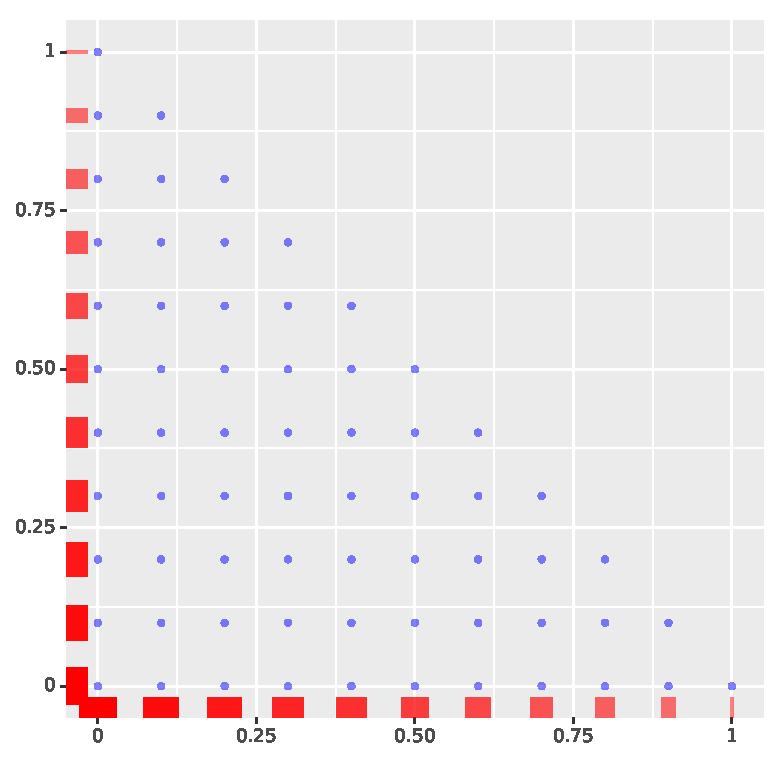
\includegraphics[scale=0.8]{dice_uprior}\hspace*{1cm}
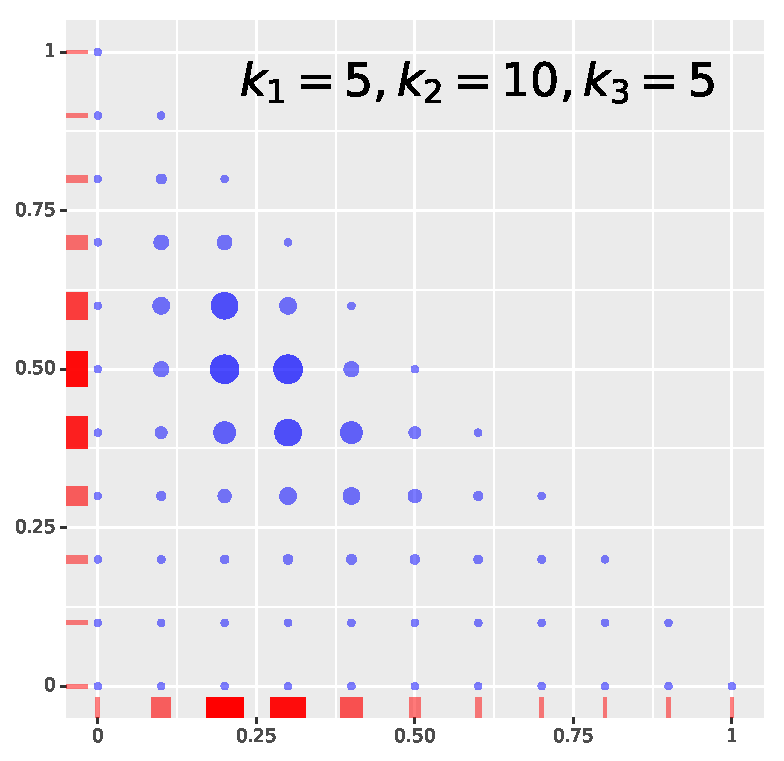
\includegraphics[scale=0.8]{dice_posterior}}

\begin{triangles}
\item Uniform prior over parameter pairs yields non-uniform marginal priors.
\item The joint MAP estimate coincides with the marginal MAP estimates.  
\end{triangles}


\foilhead[-1cm]{Dirichlet distribution as a posterior}

By increasing the number of grid points in the non-informative prior over simplex we reach a continuous distribution with a density function
\begin{align*}  
p[p_1,\ldots, p_m|k_1,\ldots, k_m] = \frac{\Gamma(n+m)}{\Gamma(k_1+1)\cdots\Gamma(k_m+1)}\cdot p_1^{k_1}\cdots p_m^{k_m}\enspace.
\end{align*}
This distribution is known as \emph{Dirichlet  distribution}
\begin{align*}
 \mathsf{Dirichlet}(\alpha_1=k_1+1,\ldots, \alpha_m=k_m+1)\enspace.
\end{align*} 
The parameter value that maximises the posterior is 
\begin{align*}
p_i^* =\frac{\alpha_i-1}{\alpha_1+\ldots\alpha_m-m}=\frac{k_i}{n}\enspace.
\end{align*} 


\foilhead[-1cm]{Laplace smoothing}

Assume that we throw a dice with $m$ faces and $B_i$ encodes the event that the dice lands on a specific face. Then it is natural to assign the maximum prior probability to the parameter value $p_*=\frac{1}{m}$.
\vspace*{1cm}

Such prior can be defined through a following though experiment:
\begin{triangles}
\item We start with non-informative prior.
\item We observe all possible outcomes of the dice $\alpha$ times.
\item We use the resulting posterior as a prior for real observations. 
\end{triangles}
\vspace*{1cm}

Thus the posterior can be obtained by starting with non-informative prior and observing $k+\alpha$ ones among $n + m\alpha$ throws.  
\begin{triangles}
\item The ratio $p=\frac{k+\alpha}{n+m\alpha}$ is the maximal aposteriori estimate for $p$.
\end{triangles}

\end{document}

\foilhead[-1cm]{Markov chains}

\textbf{Definition.}
Markov chain with order $m$ is an outcome of a process that outputs correlated observations $X_1, X_2,\ldots$ in such a way that the probability of the observation $X_{m+i}$ depends only on the observations $X_{m+i-1},\ldots, X_{m}$

\textbf{Log-likelihood.} Let $\vec{x}=(x_1,\ldots, x_{m+n})$ be a sequence of observations. Then the log-likelihood $\ell[\vec{x}]$ can be expressed
\begin{align*}
\ell[\vec{x}]=\log \underbrace{\pr{x_1,\ldots,x_m}}_{\beta[x_1,\ldots,x_m]} + \sum_{i=1}^n \log \underbrace{\pr{x_{m+i}|x_{m+i-1},\ldots, x_i}}_{\alpha[x_i,\ldots, x_{i+m-1}, x_{m+i}]} 
\end{align*}
where 
\begin{triangles}
\item the tensor $\beta[\ldots]$ determines initial probabilities;
\item the tensor $\alpha[\ldots]$ determines transition probabilities. 
\end{triangles}

\foilhead[-1cm]{Reduction to the dice throwing experiment}

Let $k(u_1,\ldots,u_{m+1})$ is the count of subsequences $u_1,\ldots,u_{m+1}$ then 
\begin{align*}
\ell[\vec{x}]=\log \beta[x_1,\ldots,x_m] + \sum_{\vec{u}} k(\vec{u})\log\alpha[\vec{u}] 
\end{align*}
Let us assume that the posterior is defined
\begin{triangles}
\item fixing probabilities for slices $\alpha[u_1,\ldots,u_{m}, *]$
\item multiplying these probabilities to get the probability of $\alpha[\ldots]$
\end{triangles}
\vspace*{1cm}

The logarithm of the posterior decomposes into sum of independent terms
\begin{align*}
\sum_{u_{m+1}} k(u_1,\ldots,u_{m+1})\cdot\log \alpha[u_1,\ldots,u_{m+1}]+ \log p(\alpha[u_1,\ldots,u_{m}, *])
\end{align*}
This is equivalent to inferring probabilities in a dice throws \vspace*{-2ex}

\foilhead[-1cm]{Hidden Markov models}

\textbf{Definition.}
Let $X_1,X_2,\ldots$ be hidden states that form a Markov chain and let $Y_1,Y_2,\ldots$ be observations that the probability of $Y_i$ depends only on the state $X_i$. Then the entire process is known as Hidden Markov Model.

\textbf{Log-likelihood.} Let $\vec{y}=(y_1,\ldots, y_{m+n})$ and $\vec{x}=(x_1,\ldots, x_{m+n})$ be the  observations and hidden states. Then the complete log likelihood is
\begin{align*}
\ell[\vec{x},\vec{y}]=\log \beta[x_1,\ldots,x_m] &+ \sum_{i=1}^n \log \alpha[x_i,\ldots, x_{i+m-1}, x_{m+i}] 
+\log \delta[x_i,y_i]
\end{align*}
where 
\begin{triangles}
\item the tensor $\beta[\ldots]$ determines initial probabilities;
\item the tensor $\alpha[\ldots]$ determines transition probabilities;
\item the tensor $\delta[\ldots]$ determines emission probabilities.
\end{triangles}


\foilhead[-1cm]{Reduction to the previous building blocks}

The problem simplifies when we know the vector of hidden states $\vec{x}$: 
\begin{triangles}
\item Inference of emission probabilities $\delta[\ldots]$ reduce to dice throwing.
\item Inference of the chain parameters $\alpha[\ldots]$ and $\beta[\ldots]$ is also possible.
\end{triangles}
\vspace*{2ex}

We can use Viterbi algorithm for finding the most probable hidden state $\vec{x}$ is easy if all parameters are known.
\vspace*{2ex}


\textbf{Naive inference algorithm:} Fix random parameters and repeat steps:
\begin{triangles}
\item Given parameters $\alpha, \beta, \delta$  learn the most probable hidden state $\vec{x}$.
\item Given the most probable hidden state $\vec{x}$ learn model parameters $\alpha, \beta, \delta$.
\end{triangles}
\vspace*{2ex}
This algorithm overfits as all hidden states can have similar probability. 


\foilhead[-0cm]{Model behind naive Bayes classifier}

\illustration[scale=0.8]{naive-bayes-scheme}

Underlying class value determines observed attributes 
\begin{triangles}
\item Each attribute $X_i$ is binary 
\item All variables are independent if class is fixed
\item Sometimes we just ignore dependancies for easier modelling
\end{triangles}

\foilhead[-0cm]{Likelihood of the data}

Let us assume that we know the probabilities
\begin{align*}
p_i&=\pr{X_i=1|Class=0}\\
q_i&=\pr{X_i=1|Class=1}
\end{align*}
Then using the independence assumption we get
\begin{align*}
\pr{X_1=a_1,\ldots,X_n=a_n|Class=0}&=\prod_{i=1}^np_i^{a_i}(1-p_i)^{1-a_i}\\
\pr{X_1=a_1,\ldots,X_n=a_n|Class=1}&=\prod_{i=1}^nq_i^{a_i}(1-q_i)^{1-a_i}
\end{align*}

\foilhead[-1cm]{Prior and posterior for the class labels}

\enlargethispage{1.5cm}
Now it is straightforward to derive
\begin{align*}
\pr{Class=0|\vec{X}=\vec{a}}&= \frac{\prod\limits_{i=1}^np_i^{a_i}(1-p_i)^{1-a_i}\cdot\pr{Class=0}}{\pr{\vec{X}=\vec{a}}}\\
\pr{Class=1|\vec{X}=\vec{a}}&= \frac{\prod\limits_{i=1}^nq_i^{a_i}(1-q_i)^{1-a_i}\cdot\pr{Class=1}}{\pr{\vec{X}=\vec{a}}}
\end{align*}
which gives an \emph{odd ratio} 
\begin{align*}
\frac{\pr{Class=0|\vec{X}=\vec{a}}}{\pr{Class=1|\vec{X}=\vec{a}}}&=\frac{\pr{Class=0}}{\pr{Class=1}}\cdot\frac{\prod\limits_{i=1}^np_i^{a_i}(1-p_i)^{1-a_i}}{\prod\limits_{i=1}^nq_i^{a_i}(1-q_i)^{1-a_i}}
\end{align*} 
 
\foilhead[-1cm]{The resulting classifier is a linear classifer}
 
By taking logarithm form the odd ratio we get
\begin{align*}
\log\left(\frac{\pr{Class=0|\vec{X}=\vec{a}}}{\pr{Class=1|\vec{X}=\vec{a}}}\right)&= w_0+\sum_{i=1}^n w_ia_i
\end{align*} 
where 
\begin{align*}
w_0&=\log\left(\frac{\pr{Class=0}}{\pr{Class=1}}\right)+\sum_{i=1}^n\log\left(\frac{1-p_i}{1-q_i}\right)\\
w_i&=\log \left(\frac{p_i}{1-p_i}\cdot\frac{1-q_i}{q_i}\right) 
\end{align*}

\foilhead[-1cm]{How to train the classifier?}
A frequentistic approach is to fix probabilities from the training sample
\begin{align*}
p_i&=\frac{\#\set{\text{data points form class 0 with $X_i=1$}}}{\#\set{\text{data points form class 0}}}\\
q_i&=\frac{\#\set{\text{data points form class 1 with $X_i=1$}}}{\#\set{\text{data points form class 1}}}
\end{align*}
However if some value does not occur for $X_i$ in the training sample we get overly confident results. Thus, Bayesian mean estimate is better alternative  
\begin{align*}
p_i&=\frac{\#\set{\text{data points form class 0 with $X_i=1$}}+1}{\#\set{\text{data points form class 0}}+2}\\
q_i&=\frac{\#\set{\text{data points form class 1 with $X_i=1$}}+1}{\#\set{\text{data points form class 1}}+2}
\end{align*}

\end{document}

\foilhead[-1cm]{Going beyond naive Bayesian models}
\illustration[scale=0.8]{bayesian-network}

Complex causal models are often defined through Bayesian networks
\begin{triangles}
\item A complex processes is first split into sub-events
\item Direct causal dependencies between sub-events are detected
\item Causation mechanisms are characterised with probability tables
\end{triangles} 
  
\foilhead[-1cm]{Strength and weaknesses of Bayesian networks}

\textbf{Strengths}
\begin{triangles}
\item Bayesian networks are easy to interpret
\item Bayesian networks are good for formalising fuzzy background knowledge
\item Estimation of individual probability tables is tractable
\item There are tools for doing inference with Bayesian networks  
\end{triangles}
\vspace*{1cm}

\textbf{Weaknesses}
\begin{triangles}
\item You must know the causal structure of sub-events  
\item Identification of causal structure form data alone is very difficult
\item It is notoriously difficult to model non-trivial causal dependencies
\item Standard inference procedures often do not have closed solutions 
\end{triangles}

\end{document}
